% 近似理论:微扰

无论在一般的量子力学框架下,还是其延伸出的各种问题,比如量子多体问题、量子统计问题、量子场论问题等等,可以精确求解的本身就是少之又少. 很多时候,一些必要的近似手段才真正地发挥了大作用.

一个最成功的近似理论就是微扰理论. 假如我们对某一个体系了解的很充分,那么对这个体系在小的已知扰动(比如,由杂质或者外界场影响等等)的行为可以非常好的用微扰进行处理,得到很多十分有效的结论.

\subsection{不含时 Time-independent}

很多微扰是不含时的微扰——比如说,我的杂质就一直扔在那里了,不管你时间怎么变化我的杂质又不会消失. 这时候的微扰论实际上是比较基础的,我们不用引入很多奇葩观念就可以轻松地解决问题. 在这种时候,有一个很有趣的现象我们后面会看到.

注意到,如果微扰很小的话,微扰之后本征态的能量、态都很接近微扰之前的能量,比如说,$|n^{(0)}\rangle, E_n^{(0)}$ 分别表示原来的本征态和能量,微扰之后在它附近的能量本征态为 $|n,\lambda\rangle, E_n$,$\lambda$ 为一个描述微扰大小的参数. 所以,我们的一般想法就是:假定满足如下关系:
\begin{equation}
E_n = E_n^{(0)} + \lambda E_n^{(1)} + \lambda^2 E_n^{(2)} + \cdots\\
|\psi_n\rangle = |\psi_n^{(0)}\rangle + \lambda|\psi_n^{(1)}\rangle + \lambda^2 |\psi_n^{(2)}\rangle
\end{equation}

注意,一目了然,这并没有进行\bb{归一化}. 另外,很直观的,假定 $|\psi_n^{(k>0)}\rangle$ 与原本征态 $|\psi_n\rangle$ 正交.

\subsubsection{非简并问题}

为什么上来先强调非简并问题,这实际上在后面可以看出来. 一个比较直观的说法是这样的:如果简并了,那么我实际上在这两个简并态之间随意组合都可以得到处于该能量的本征态,尽管其中只有一些是有一定的物理意义(也就是其他算符本征态)的. 在这么多种本征态组合中,究竟哪个和微扰之后的本征态最为接近呢?这就是一个技术上的问题. 并不是不能考虑,但是在这里我们先处理点最简单的问题,在后面我们再考虑简并情况.

在进一步说明问题前,我们先考虑一个更更简单的情况:一个可以严格对角化的 $2\times2$ 问题.

\begin{exer}{}
一个体系的非微扰Hamiltonian是:
\begin{equation}
H_0 = E_1|e^0\rangle\langle e^0| + E_2|g^0\rangle\langle g^0| =  \left(\begin{matrix} E_1 & 0\\ 0 & E_2\end{matrix}\right)
\end{equation}
其中 $E_1<E_2$. 而微扰部分的Hamiltonian则是
\begin{equation}
H_1 = \lambda(|e^0\rangle\langle g^0|+|g^0\rangle\langle e^0|)
\end{equation}

显然,这是一个实对称矩阵(Hermitian矩阵),我们可以把它用一个正交矩阵(Unitary矩阵)进行对角化:
\begin{equation}
H = H_0+H_1 = U\Her\left(\begin{matrix} \lambda_- & 0\\0 & \lambda_+\end{matrix}\right)U
\end{equation}

其中,我们知道
\begin{equation}
\lambda_{\pm} = \frac{E_1+E_2}{2} \pm \sqrt{\left( \frac{E_1-E_2}{2}\right)^2 + \lambda^2}
\end{equation}

假如这个微扰后的Hamiltonian的本征态是 $(a_\pm,b_\pm)^T$,那么我们知道
\begin{equation}
U\left(\begin{matrix}a_-\\b_-\end{matrix}\right) = \left(\begin{matrix}1\\0\end{matrix}\right)\quad U\left(\begin{matrix}a_+\\b_+\end{matrix}\right) = \left(\begin{matrix}0\\1\end{matrix}\right)
\end{equation}
从而
\begin{equation}
U^T(\equiv U\Her) = \left(\begin{matrix}a_- & a_+\\b_- & b_+\end{matrix}\right), \quad U = \left(\begin{matrix}a_- & b_-\\a_+ & b_+\end{matrix}\right)
\end{equation}

而我们知道:未归一化的本征态可以写成很好的形式,即
\begin{equation}
\left(\begin{matrix}a_-\\b_-\end{matrix}\right) \propto \left(\begin{matrix}1 \\ \ \\ \displaystyle\frac{\lambda_- - E_1}{\lambda}\end{matrix}\right),\quad \left(\begin{matrix}a_+\\b_+\end{matrix}\right) \propto \left(\begin{matrix}1 \\ \ \\ \displaystyle\frac{\lambda_+ - E_2}{\lambda}\end{matrix}\right)
\end{equation}

1. 验证上式

2. 计算:如果在 $t=0$ 的时候体系处于 $|\psi(t=0)\rangle = |g^0\rangle$,那么其时间演化是怎样的

(Hint and solution of 2. :

设
\begin{equation}
\left(\begin{matrix}a_-\\b_-\end{matrix}\right) =\frac{1}{A} \left(\begin{matrix}1 \\ \ \\ \displaystyle\frac{\lambda_- - E_1}{\lambda}\end{matrix}\right),\quad \left(\begin{matrix}a_+\\b_+\end{matrix}\right) =\frac{1}{B} \left(\begin{matrix}1 \\ \ \\ \displaystyle\frac{\lambda_+ - E_1}{\lambda}\end{matrix}\right) 
\end{equation}

那么,在经过 $U$ 变换的坐标系中($|g\rangle,|e\rangle$是完整的Hamiltonian的本征态),$|\psi(t=0)\rangle = |g\rangle/A + |e\rangle/B$,一切都变得简单了起来. $|\psi(t)\rangle = \E^{-\lambda_-t/\hbar}|g\rangle/A + \E^{-\lambda_+t/\hbar}|e\rangle/B$,其中必然有 $1/A^2 + 1/B^2 = 1$(这个验算可能会比较繁琐,Mathematica结果见\autoref{AprPtr_fig1})

\begin{figure}[ht]
\centering
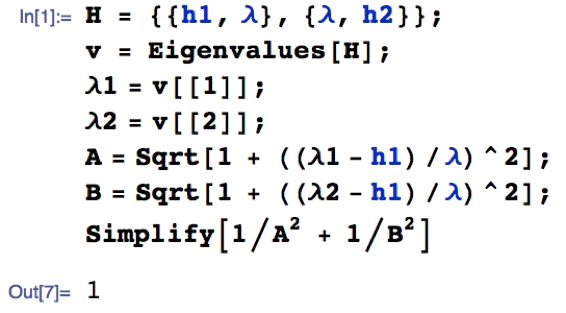
\includegraphics[width=8cm]{./figures/AprPtr1.pdf}
\caption{Tedious Calculation Check via Mathematica} \label{AprPtr_fig1}
\end{figure}

其 $|g^0\rangle,|e^0\rangle$ 的分量为
\begin{equation}
\langle g^0|\psi(t)\rangle = \E^{-\lambda_-t/\hbar}\frac{1}{A^2} + \E^{-\lambda_+t/\hbar}\frac{1}{B^2}
\end{equation}

其中,
\begin{equation}
A^2 = 1 + \left(\frac{\lambda_- - E_1}{\lambda}\right)^2 ,\quad B^2 = 1 + \left(\frac{\lambda_+ - E_1}{\lambda}\right)^2
\end{equation}

其模长的为
\begin{equation}\ali{
|\langle g^0|\psi(t)\rangle|^2 &= \frac{1}{A^4}+\frac{1}{B^4} + \frac{2}{A^2B^2}\cos((\lambda_+-\lambda_-) t/\hbar) \\
&= 1 - \frac{2}{A^2B^2}(1-\cos((\lambda_+-\lambda_-) t/\hbar))
}\end{equation}

而容易知道(via Mathematica),
\begin{equation}
\lambda_+-\lambda_- = 2\sqrt{\left( \frac{E_1-E_2}{2}\right)^2 + \lambda^2},\quad \frac{1}{A^2B^2} = \frac{\lambda^2}{(E_1-E_2)^2+4\lambda^2}
\end{equation}

于是
\begin{equation}
\begin{split}
|\langle g^0|\psi(t)\rangle|^2 &= 1 - \frac{2\lambda^2}{(E_1-E_2)^2+4\lambda^2}\left(1-\cos\left(2\sqrt{\left( \frac{E_1-E_2}{2}\right)^2 + \lambda^2}\frac{t}{\hbar}\right)\right) \\
&= 1 - \frac{4\lambda^2}{(E_1-E_2)^2+4\lambda^2}\sin^2\left(\sqrt{\left( \frac{E_1-E_2}{2}\right)^2 + \lambda^2}\frac{t}{\hbar}\right)
\end{split}
\end{equation}

)

可以做一定的物理分析:当 $E_2\to E_1$ 的时候(亦即简并情况),我们知道任何一个Hermitian的微扰之后的本征态都是 $(|g^0\rangle + |e^0\rangle)/\sqrt{2}$, $(|g^0\rangle - |e^0\rangle)/\sqrt{2}$. 在那种情况下,我们的原始态在新的态上的概率是一样的,换句话说,很有可能存在某些时候,两个振幅相同的新的态的 $|g^0\rangle$ 分量相干相消——而我们计算的解析结果也确实是这样,在那个时候,$\sin^2$ 前面的因子为 1,即确实存在某些时刻体系完全处于 $|e^0\rangle$ 上.
\end{exer}

那么,一般的非简并问题是怎么处理的呢?首先,我们要定义一些算符. 这一段可能比较枯燥,但是当你看到它的效果之后就会震惊于我们之前进行的这些步骤是多么的重要.

我们首先(重新)定义我们在“ 基本概念\upref{Basics}” 中就见到过的投影算符;不同的是,我们要对每一个态都定义如此一个投影算符:
\begin{equation}
\hat{\mathcal{P}}_n = |\psi^0_n\rangle\langle\psi^0_n|,\quad \hat{\mathcal{Q}}_n = 1-\hat{\mathcal{P}}_n 
\end{equation}

显然有
\begin{equation}
\hat{\mathcal{P}}_n \hat{\mathcal{Q}}_n = \hat{\mathcal{Q}}_n \hat{\mathcal{P}}_n =0,\quad [\hat{\mathcal{P}}_n ,H_0] = [\hat{\mathcal{Q}}_n ,H_0] = 0
\end{equation}

考虑定态的薛定谔方程 $(H_0+\lambda \hat{V})|\psi_n\rangle = E_n|\psi_n\rangle$,我们首先把 $|\psi_n\rangle$ 拆成与原本正交的部分和与原本重合的部分,也就是说
\begin{equation}
|\psi_n\rangle = \hat{\mathcal{P}}_n|\psi_n\rangle + \hat{\mathcal{Q}}_n|\psi_n\rangle
\end{equation}

其中呢,第二项是很小的微扰项,需要去求解. 我们把薛定谔方程按照此思路重新展开. 先看左边,
\begin{equation}
\begin{split}
\text{left} &= \hat{H}_0\hat{\mathcal{P}}_n|\psi_n\rangle + \lambda \hat{V}\hat{\mathcal{P}}_n|\psi_n\rangle + \hat{H}_0\hat{\mathcal{Q}}_n|\psi_n\rangle + \lambda \hat{V}\hat{\mathcal{Q}}_n|\psi_n\rangle\\
&=E_n^{(0)}\hat{\mathcal{P}}_n|\psi_n\rangle + \lambda \hat{V}\hat{\mathcal{P}}_n|\psi_n\rangle + \hat{H}_0\hat{\mathcal{Q}}_n|\psi_n\rangle + \lambda \hat{V}\hat{\mathcal{Q}}_n|\psi_n\rangle
\end{split}
\end{equation}

而右边可以展开成
\begin{equation}
\begin{split}
\text{right} &= E_n\hat{\mathcal{P}}_n|\psi_n\rangle + E_n\hat{\mathcal{Q}}_n|\psi_n\rangle
\end{split}
\end{equation}

这两个相等,也就是说
\begin{equation}\ali{
&E_n^{(0)}\hat{\mathcal{P}}_n|\psi_n\rangle + \lambda \hat{V}\hat{\mathcal{P}}_n|\psi_n\rangle + \hat{H}_0\hat{\mathcal{Q}}_n|\psi_n\rangle + \lambda \hat{V}\hat{\mathcal{Q}}_n|\psi_n\rangle\\
&= E_n\hat{\mathcal{P}}_n|\psi_n\rangle + E_n\hat{\mathcal{Q}}_n|\psi_n\rangle
}\end{equation}

从而得到
\begin{equation}\label{AprPtr_eq21}
(E_n - \hat{H}_0)\hat{\mathcal{Q}}_n|\psi_n\rangle = (E_n^{(0)}-E_n)\hat{\mathcal{P}}_n|\psi_n\rangle+\lambda \hat{V}|\psi_n\rangle
\end{equation}

将 $\hat{\mathcal{Q}}$ 左乘\autoref{AprPtr_eq21}, 我们得到
\begin{equation}\ali{
\hat{\mathcal{Q}} (E_n - \hat{H}_0)\hat{\mathcal{Q}}_n|\psi_n\rangle &= \hat{\mathcal{Q}}(E_n^{(0)}-E_n)\hat{\mathcal{P}}_n|\psi_n\rangle+\hat{\mathcal{Q}}\lambda \hat{V}|\psi_n\rangle \\
&= 0 +\hat{\mathcal{Q}}\lambda \hat{V}|\psi_n\rangle
}\end{equation}

而显然 $\hat{\mathcal{Q}} = \hat{\mathcal{Q}}\hat{\mathcal{Q}}$,从而得到
\begin{equation}
\hat{\mathcal{Q}} (E_n - \hat{H}_0)\hat{\mathcal{Q}}_n\hat{\mathcal{Q}}|\psi_n\rangle = \lambda\hat{\mathcal{Q}} \hat{V}|\psi_n\rangle
\end{equation}

\subsection{含时 Time-dependent}

\subsubsection{问题分析:原子自发辐射}

我们接下来分析原子自发辐射问题来回顾我们这一章学过的东西. 问题背景:我们考虑部分量子化了的原子—光相互作用,其 Hamiltonian 可以用如下方程描述(已经经过部分简化,如偶极近似,旋波近似):
\begin{align}
\begin{split}
H &= H_0+H_{int},\\
H_0 &= \sum_{\vec k}\hbar\omega_{\vec k}a\Her_{\vec k}a_{\vec k} + \frac{1}{2}\hbar\omega_{eg}\sigma_z,\\
H_{int} &= \hbar\sum_{\vec k} \Omega_{\vec k}\sigma_+ a_{\vec k} \E^{\I\vec k\cdot r} + \Omega_{\vec k}^*\sigma_- a_{\vec k}\Her \E^{-\I\vec k\cdot r} .
\end{split}
\end{align}

其中,$\omega_{eg}$ 表示从激发态 $|e\rangle$ 跃迁到基态 $|g\rangle$ 的光子的角频率,$\hbar\Omega_{\vec k} \equiv -e\langle e|{\vec r}|g\rangle\cdot \hat\epsilon_{\vec k}\varepsilon_{\vec k}$ 总之就是一个频率量纲的东西并不重要, $a_{\vec k} = a_{\vec k}(t) = a_{\vec k,0} \E^{-\I\omega t}$.

\begin{exer}{}
我们试图引入相互作用汇景,
\begin{equation}
H^I(t) = \E^{\I H_0t/\hbar} H_{int} e^{-\I H_0t/\hbar}
\end{equation}

明显,会带来 nontrivial 的项的是如下两项
\begin{equation}\ali{
&\E^{\I\omega_{\vec k}a\Her_{\vec k}a_{\vec k}t}a_{\vec k} \E^{-\I\omega_{\vec k}a\Her_{\vec k}a_{\vec k}t} = a_{\vec k} \E^{-\I\omega_{\vec k}t}\\
& \E^{i\omega_{eg}\sigma_zt/2}\sigma_+ \E^{\I \omega_{eg}\sigma_zt/2} = \sigma_+ \E^{-\I\omega_{eg}t}
}\end{equation}

试推导这两个式子,并进而写出 Hamiltonian $H^I(t)$.
\end{exer}

我们有
\begin{equation}
H^I(t) = \hbar\sum_{\vec k}\left[\Omega_{\vec k}\sigma_+a_{\vec k} \E^{\I(\omega_{eg}-\omega_{\vec k})t} + h.c.\right]
\end{equation}